\Large\textbf{Capitolo 3: \\ Struttura della membrana}

\section{Lipidi}
\small
    I lipidi sono una classe di biomolecole che sono caratterizate da una porzione idrofoba. 
    
    \subsection{Acidi grassi}
        Gli acidi grassi sono una categoria di lipidi caratterizzati da una catena idrocarburica più o meno lunga. Qualora compaiano doppi legami tra i carboni della coda, si dice che l'acido grasso è \textit{insaturo}, si dice \textit{saturo} altrimenti. La presenza di code insature favoriscono il comportamento liquido della membrana, al contrario, la presenza di catene insature favoriscono al rigidità.
        
    \subsection{Fosfolipidi}
        I fosfolipidi sono una classe di lipidi composti da due catene idrocarburiche e una testa di glicerolo: la testa è fortemente idrofila mentre la coda fortemente idrofobica.
        Questa struttura conferisce la caratteristica \textit{anfipatica} alla molecola.\\
        La \textit{fosfatidilcolina} è il fosfolipide più abbondante nelle membrane, è composto di colina, fosfato, glicerolo e due code idrofobiche.
        \subsubsection{Fosfogliceridi}
            Sono una categoria di fosfolipidi che si differenziano tra loro in base alla composizione della testa polare, alla quale di aggiunge il di-acil-glicerolo. Tra queste possiamo ricordare \textit{fosfatidil serina}, \textit{fosfatidil inositolo} e \textit{fosfatidil colina}.
            
        \subsubsection{Plasmalogeni}
            Sono una sottoclasse di fosfolipidi caratterizzata da un gruppo vinil-etere in posizione 1 del glicerolo. Le catene idrocarburiche sono legate una tramite un legame etere e una tramite legame estere.
        
    \subsection{Trigliceridi}
        Sono una categoria di lipidi scarsamente anfipatica, proprio per questo motivo non fanno parte della membrana cellulare.
        
    \subsection{Sfingolipidi}
        Sono una categoria di lipidi simili ai fosfolipidi, al posto del glicerolo contengono sfingosina e una testa polare, al quale è legata una catena acida, un gruppo amminico e due gruppi ossidrili. Sono anche esse molecole anfipatiche. ???
        
    \subsection{Steroli}
        Sono una categoria di lipidi presenti negli animali (gli analoghi vegetale sono ergosterolo e stigmasterolo).
        Sono composti da quattro anelli idrocarburici e una coda idrocarburica non polare.\\
        Anche questa categoria presenta caratteristiche anfipatiche dovute alla presenza di un gruppo ossidrile dal lato opposto della catena.\\
        Sono di dimensioni inferiori rispetto ai fosfolipidi, sono presenti nel doppio strato lipidico della membrana: il gruppo OH dello sterolo interagisce con la testa polare dei fosfolipidi e costituiscono una componente più interna.\\
        La funzione di queste molecole all'interno della membrana è legata alla fluidità del mosaico: una maggior concentrazione aumenta la rigidità (nel caso si introducano artificialmente si assiste al comportamento inverso).
        
    \subsection{Glicolipidi}
        I glicolipidi sono una categoria di lipidi che contengono uno zucchero come residuo legato alla testa polare. Sono presenti solo nello strato esterno della membrana. L'aggiunta dello zucchero avviene a livello del Golgi. \\
        La loro funzione comprende l'interazione tra la cellula e l'ambiente, sono punti di ingresso per tossine e sono utili per cariche elettriche e pH. ???
    
\section{Doppio strato lipidico}
    La membrana plasmatica consiste di un doppio strato lipidico, formato prevalentemente da fosfogliceridi, steroli, glicolipidi e sfingolipidi. Tra questi i primi sono i più abbondanti.\\
    La struttura planare di doppio strato lipidico è energicamente sfavorita, se la si pone in soluzione infatti tenderà a richiudersi su se stessa formando un liposoma chiuso (detti micelle qualora non contengano all'interno soluzione acquosa).
    \vspace{0.5cm}
    I vari tipi di lipidi sono presenti in percentuali differenti in porzioni della membrana differenti. Per esempio la sfingomielina è presente al 13\% nelle membrane mieliniche mentre si limita all'8\% nel Golgi e al 3\% nel RE.
    Fosfatidil etanolammina e fosfatidil serina sono invece presenti solo a livello del figlietto citosolico. 
    Al contrario, fosfatidil colina e sfingomielina sono presenti solo a livello del foglietto esoplasmatico.
    Questo suggerisce che i lipidi vengano aggiunti alla membrana e successivamente spostati (a livello di foglietto) da componenti dedicate.
    \subsection{Spostamenti dei lipidi di membrana}
        I lipidi di membrana possono effettuare degli spostamenti di tre tipi:
        \begin{enumerate}
            \item diffusione laterale: si fanno spazio tra i lipidi adiacenti
            \item rotazione sul proprio asse verticale
            \item flip-flop: cambiano il foglietto (da interno a esterno o viceversa).
        \end{enumerate}
        Quest'ultima tipologia di movimento è molto rara se la si considera isolatamente. Tuttavia esistono degli enzimi che catalizzano questo movimento, quali \textit{scramblasi} e \textit{flippasi}.
        \subsubsection{Scambrlasi e flippasi}
            La scramblasi è un enzima lipide-specifico che serve ad ababssare l'energia di attivazione per il flip-flop. \\
            La flippasi è un enzima che idrolizza ATP per promuovere l'asimmetria di lipidi specifici. \\
            Queste due molecole insieme determinano la distribuzione dei lipidi di membrana. Sono coinvolte anche nel caso in cui una cellula debba andare incontro a morte programmata: viene infatti promossa una asimmetria di fosfatidil serina, quindi viene riconosciuta da macrofagi e viene eliminata.
        
    \subsection{Volumi e disposizioni}
        Diverse tipologie di fosfolipidi occupano volumi differenti a seconda della loro composizione. In particolare:
        \begin{itemize}
            \item fosfatidil colina occupa un volume cilindrico
            \item fosfatidil etanolammina occupa un volume assimilabile ad un cilindro, la cui testa occupa il vertice
            \item sfingomielina occupa un volume cilindrico in altezza superiore alla fosfatidil colina
        \end{itemize}
        
        \begin{figure}[h]
            \centering
            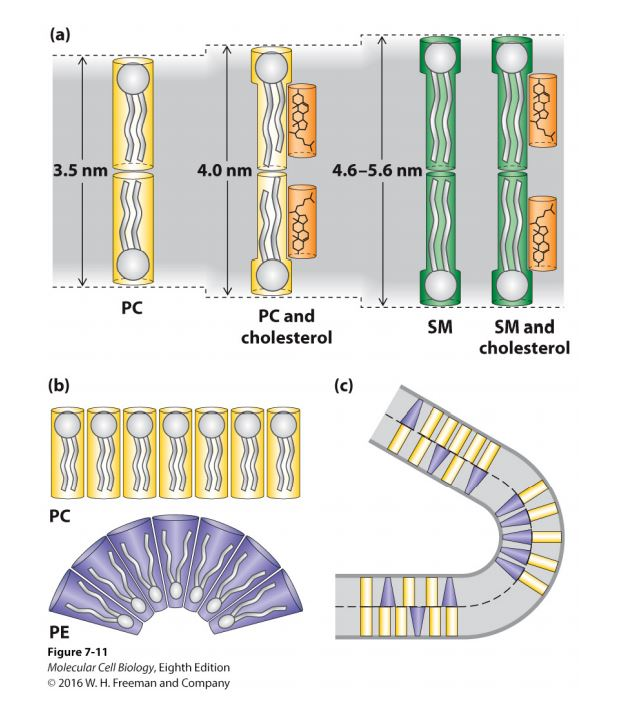
\includegraphics[width=0.5\textwidth]{images/doppiostrato.JPG}
            \caption{\small volume della membrana in relazione a lipidi differenti}
            \label{fig:mesh1}
        \end{figure}
        
        In base alle componenti dei foglietti lipidici, la membrana assume conformazione e spessore differente:
        \begin{itemize}
            \item un doppio strato di fosfatidil serina combinato con degli steroli aumenta lo spessore rispetto a un doppio strato di fosfatidil serina semplice
            \item un doppio strato di sfingomielina combinato con degli steroli \textit{non} aumenta lo spessore rispetto a un doppio strato di sfingomielina semplice. Essendo la sfingomielina \textit{un cilindro più alto}, questo doppio strati risulta più spesso di quello di fosfatidil serina.
            \item la presenza di fosfatidil etanolammina induce un ripiegamento.
        \end{itemize}

        Esistono processi che permettono una temporanea formazione di zattere lipidiche (composizione specifica locale di lipidi) per specializzazioni della membrana.\\
    
\section{Proteine di membrana}
    \small
    Ogni membrana incorpora delle proteine con funzionalità specifiche.
    \subsection{Tipologie di proteine di membrana}
        Le proteine di membrana possono essere integrali, ancorate a lipidi o periferiche di membrana. Molto raramente si può trattare di un $\alpha E$ associata ad un mono-strato.
        
         \begin{figure}[h]
            \centering
            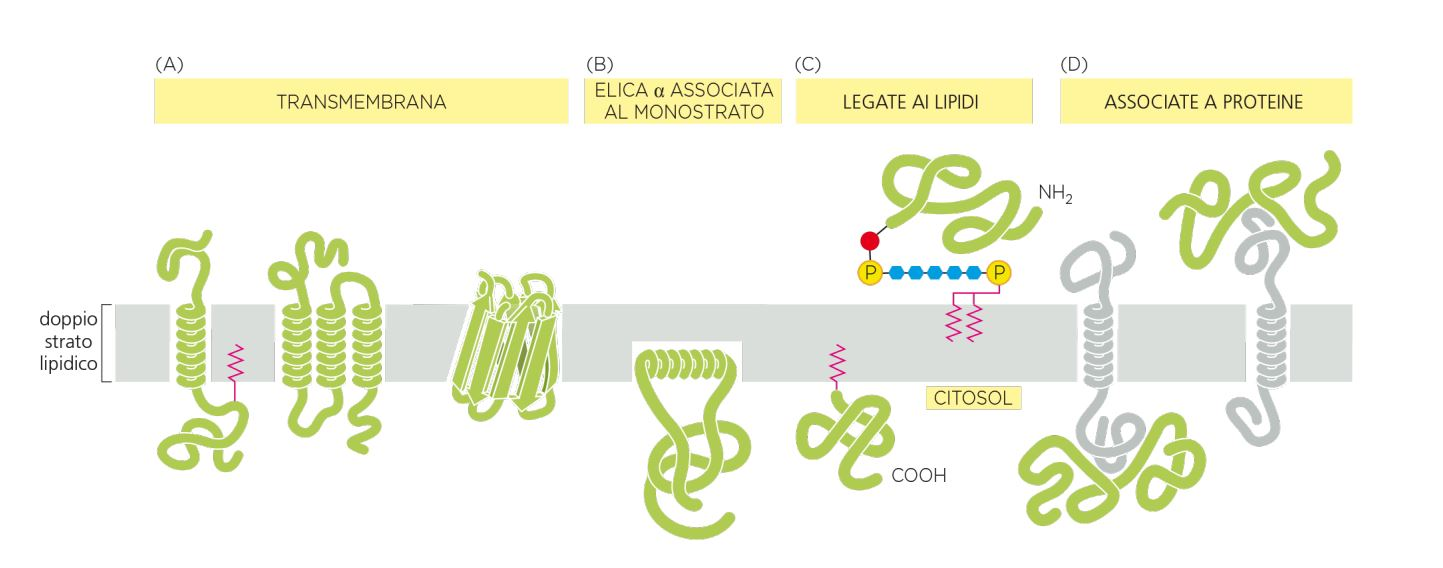
\includegraphics[width=1\textwidth]{images/proteinemembrana.JPG}
            \caption{\small tipologie di proteine di membrana}
            \label{fig:mesh1}
        \end{figure}
        
        \subsubsection{Integrali di membrana}
            Consistono di tre domini:
            \begin{enumerate}
                \item transmembrana: la porzione che effettivamente attraversa il doppio strato lipidico.
                \item luminale o extracellulare: il dominio che volge sul lumen o all'esterno della cellula
                \item citosolico: la parte che si interfaccia con il citosol
            \end{enumerate}
            Attraversano da parte a parte la membrana una (\textit{single pass}) o più volte (\textit{multi pass}) la membrana cellulare. Un passaggio è composto di un elica di circa 20/25 AA (a seconda della composizione della membrana attraversa spessori differenti).\\
            Una proteina single-pass termina solitamente con le cariche negative volte verso il lumen o porzione extracellulare e la porzione positiva verso il citosol.\\
            Di seguito degli esempi di proteine transmembrana costituite di $\alpha E$:
            \begin{itemize}
                \item {Glicoforina a dimero}:
                La struttura di questa proteina presa singolarmente attraversa la membrana tramite una sola $\alpha E$, la sua struttura quaternaria è composta di due di queste molecole.
                L'associazione di due proteine è promossa dall'interazione delle due $\alpha -E$ per formare un coiled-coil transmembrana.
                \item{Acuaporina}:
                L'acquaporina è un esempio di proteina multipass: la struttura terziaria è composta di sei $\alpha E$ transmembrana diagonali ad essa, quella quaternaria comprende quattro di questi domini e permette la formazione di canali acquosi.
                \item{Rodopsina}:
                La rodopsina è un esempio di proteina multipass composta di sette $\alpha E$ transmembrana perpendicolari ad essa.
                \item{TRC (\textit{T-cell-receptor})}:
                è una struttura che consiste di complessi carichi che si associano perchè energicamente favoriti.
            \end{itemize}
            Un canale transmembrana costituito di $F\beta$ sono le porine: sono strutturate a $\beta barile$, le componenti transmembrana sono idrofiliche verso l'interno e idrofobiche verso l'esterno. Generalmente le proteine di membrana con $F\beta$ sono più rigide.
            
        \subsubsection{Ancorate a lipidi}
            Le proteine ancorate ai lipidi non possiedono una porzione proteica ancorata al doppio strato, bensì sono solamente affacciati sul citosol o sulla porzione extracellulare.
            Sono tipicamente globulari, possiedono una componente idrofilica e sono covalentemente legate ai lipidi tramite una delle seguenti reazioni:
            \begin{itemize}
                \item alcilazione
                \item prenilazione
                \item GPI anchor (\textit{glicosil fosfatidil inositolo}, un glicolipide, componente saccaridica si lega alla proteina), tipicamente extracellulari
            \end{itemize}
            
        \subsubsection{Periferiche di membrana}
            Sono associate temporaneamente alla membrana tramite legami non covalenti, per esempio possono associarsi ad altre proteine transmembrana. Esistono diverse fosfolipasi che idrolizzano legami differenti. Sono usate sperimentalmente su cellule intatte per verificare la composizione del foglio esterno della membrana. Enzimi idrofili?
        
        \subsubsection{Proteine e lipidi glicosilati}
            A livello della membrana sono comprese anche proteine e lipidi associati alla membrana glicosilati. \\
            Nelle cellule eucariotiche il \textit{cortex} è costituito in larga parte di \textit{spettrina} che forma reticolo sulla faccia citoplasmatica che si associa ad altre proteine transmembrana e ne conferisce determinate proprietà meccaniche.\\
            Ad esempio i gruppi sanguigni umani sono oligosaccaridi ancorati sul lato extracellulare della membrana. Hanno una configurazione di base alla quale possono aggiungersi precisi monosaccaridi per determinare i gruppi A o B. 
            
    \subsection{Detergenti}
        Al fine di studiare le componenti proteiche facenti parte della membrana cellulare, è possibile utilizzare un detergente per estrarle tramite solubilizzazione con un \textit{detergente}.\\
        I detergenti sono sostanze anfipatiche che stabilizzano la porzione idrofoba della proteina. Possono essere ionici o non-ionici.
        \subsubsection{Ionici}
            Sono detergenti "aggressivi", talvolta sono troppo efficaci al fine dell'estrazione della proteina e possono portare alla denaturazione della proteina. Formano una micella attorno alla proteina. Un esempio è \textit{SDS}, che ha carica netta e viene associato ad uno ione.
        \subsubsection{Non-ionici}
            Sono detergenti con una polarità ma non una carica netta, questo permette di evitare la denaturazione della proteine, dissolvendo le proteine ma non formando micelle nette. 
            Sopra una certa concentrazione del detergente anche in questo caso di va incontro alla formazione di una micella: si parla ci \textit{CMC}, ovvero \textit{critical mycell concentration}.
        
    \subsection{Studio delle proteine di membrana}
        \subsubsection{FRAP}
            FRAP (\textit{fluorecence recovery after photoblieaching}) è una tecnica che si può usare sperimentalmente per verificare la migrazione dei lipidi sulla membrana. \\
            Il processo consiste nel marcare una determinata zona della membrana cellulare con fluorescenza. Applico un bleaching in un dominio di membrana limitato ("spegnendo" la fluorescenza localmente) e osservo nel tempo la ricomparsa della fluorescenza in quella zona.\\
            La ricomparsa della fluorescenza in rapporto al tempo indica la capacità di migrazione dei lipidi attraverso la membrana, ovvero il \textit{coefficente di diffusione}.
        \subsubsection{SPT o SMT}
            SPT o SMT (\textit{single particle/molecule tracking}) è una tecnica per visualizzare il movimento di una singola molecola nel tempo.\\
            Analizzandone il tracciato si può dedurre se una molecola è libera o ha una bassa motilità.
        
\pagebreak